% !TEX root = rosaryv2.tex
% !TEX recipe = LuaLaTeX+se
%\documentclass{article}
\documentclass[parskip]{scrartcl} % set document class: manual at https://ctan.org/pkg/koma-script
%\usepackage{fontspec}

% Load packages:
\usepackage[osf,p]{libertine} % set font
\usepackage[autocompile]{gregoriotex} % enable Gregorio score inclusion
\usepackage[latin]{babel} % set language
\usepackage{multicol}
\usepackage[margin=3cm]{geometry}
\usepackage{scrlayer-scrpage}
%\usepackage{musixtex}

\newcommand{\myhome}{C:/Users/johna/Chant/}
\gresetgregpath{{\myhome}}

\setkomafont{section}{\normalfont\centering\huge\scshape} % section heading style
\setkomafont{subsection}{\normalfont\centering\Large\scshape} % section heading style
\setkomafont{subsubsection}{\normalfont\centering\small\scshape} % section heading style
%\setcounter{secnumdepth}{-\maxdimen} % remove section numbering

\setkomafont{pagehead}{\scshape}
\automark[section]{section}
%\automark*[subsection]{subsection}

%\lohead[\thesection]
%{\thesection}
%\rohead[\thesubsection]
%{\thesubsection}
\pagestyle{scrheadings}

\def\translation{NABRE}

% Set the space around the initial:
% See http://gregorio-project.github.io/gregoriotex/details.html for more details and options
\grechangedim{beforeinitialshift}{2.2mm}{scalable}
\grechangedim{afterinitialshift}{2.2mm}{scalable}

% Set the initial font (change 43 for a larger size):
%\grechangestyle{initial}{\fontsize{43}{43}\selectfont}%

% Make staff lines red; remove for black:
%\gresetlinecolor{gregoriocolor}

% Use the "commentary" field of the score in the top right corner:
\gresetheadercapture{commentary}{grecommentary}{string}

% Format annotation above initial
\grechangestyle{annotation}{\small\bfseries}

\begin{document}

\section{Common Prayers}
    \subsection{The Our Father}

        \subsubsection{Simple Tone}
        \gregorioscore{Communes/pater-noster/English-ferialis}~\label{pater:simple}

        \subsubsection{Tone A.}
        \gregorioscore{Communes/pater-noster/English-A}~\label{pater:A}

        \subsubsection{Tone C.}
        \gregorioscore{Communes/pater-noster/English-C}~\label{pater:C}

    \subsection{The Hail Mary \& Glory Be}
        \paragraph{The ``classic'' Ave Maria chant}
        I use the following chant for the three Hail Marys at the
        beginning of the Rosary.~\label{avemaria}
        \gregorioscore{Varia/ave-maria/solesmes}

        The matching Gloria Patri is below.
        \gregorioscore{Rosary/Gloria/1-solemn}

        \paragraph{According to Psalm Tones}
        In this book, we sing the decades of the Rosary in the
        manner of chanting the Divine Office, using the
        Psalm tones.
        Which tone to use is dictated by the \emph{antiphon} that is
        sung before and after the decade.

        For example, the formula for Tone 8---one
        of the more common tones---is:
        \gregorioscore{Rosary/Tones/viii}
        The parts of a tone are as follows:
        \begin{itemize}
            \item \emph{Sic incipitur}--the \emph{``intonation''}.
                In the Divine Office, this part is typically only
                sung for the \emph{first} verse of a psalm, and in
                deference to that tradition, this book recommends only
                singing the intonation for the first Hail Mary of each decade.
            \item \emph{et sic flectitur}--some psalm verses (and both halves of the Hail Mary)
                have three lines, in which case the first ends like this.
            \item \emph{et sic mediatur}--how to sing the first half of a 
                typical two-line psalm verse, or the second line of a longer
                psalm verse.
            \item \emph{atque sic finitur}--how to sing the last line of
                each verse. 
        \end{itemize}
        \paragraph{Which tone do I use?} 
        There are eight numbered Gregorian psalm tones, and a few others
        (this book includes \emph{tonus peregrinus} which is not one of the
        usual eight.) Moreover, notice that in tone 8 above there is a choice
        of ending! The tone---and ending---are dictated by the antiphon,
        as follows:

        \begin{center}
            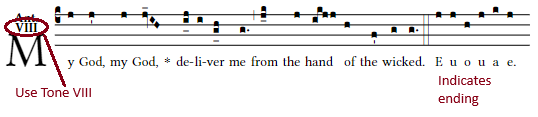
\includegraphics[width=0.8\textwidth]{Rosary/antiphon.png}            
        \end{center}

        \subsection{The Psalm tones}
        

        I have chosen the ICET translation of the Glory Be that is used
        in the American English Liturgy of the Hours (at least as of 2024.)

        \paragraph{Tone 8}~\label{ave:8c}\\
        The formula for Tone 8 is:
        \gregorioscore{Rosary/Tones/viii}

        \subsubsection{Hail Mary---tone VIII}\label{ave:examples}
        \gregorioscore{rosary/Aves/8c}

        The first two notes are called the \emph{intonation} and
        are only sung for the first Hail Mary of the decade.
        Subsequent Hail Marys begin on the tenor (held) note:
        \gresetinitiallines{0}
        \gabcsnippet{
            <i>2-10.</i> Hail(j) Ma(j)ry,(j) full(j) of(j) grace...(j) (::Z)
        }
        \gresetinitiallines{1}


    \subsection{O My Jesus}~\label{prayer:Jesus}
        \gabcsnippet{
            (c3)O,(h) my(h) Jesus!(h) For(h)give(h) us(g) our(f) sins;(h.) (;)
            save(h) us(h) from(h) the(h) fires(h) of(d) hell.(d.) (:)
        }
        \gresetinitiallines{0}
        \gabcsnippet{
            (c3)<sp>R/</sp>. <b>Lead(h) all(h) souls(h) to(h)
            hea(gf)ven(h.) (;) esp(h)ec(h)ial(h)ly(h) those(h)
            in(h) most(h) need(h) of(h) thy(h) mer(h.)cy.</b>(d.) (::)
        }
        \gresetinitiallines{1}


\clearpage
\section{The Rosary in Simple Tones}
    \emph{This section is intended for:}
    \begin{itemize}
        \item \emph{Beginners;}
        \item \emph{Penitential days; e.g.,
            Fridays outside of the Christmas and Easter seasons,
            Lenten weekdays.}
    \end{itemize}
    \emph{The Our Father, O My Jesus, and tone for the announcing of the mystery
    are among the simplest. The antiphons are no simpler than those given
    in the Intermediate Tones section following, but in this section
    are all taken from Modes II and VIII. The antiphons given here 
    can certainly also be mixed \& matched with those given in 
    Intermediate Tones.}

    \begin{center}
        \textbf{Begin:} \emph{In the Name of the Father, and of the Son,
            and of the Holy Spirit. Amen.}
    \end{center}

    Apostle's Creed, silently or \emph{recto tono}.

    Our Father, simple tone, pg.~\pageref{pater:simple}.

    Three Hail Marys, pg.~\pageref{avemaria}.


    \subsection{The Joyful Mysteries}

        %%%%%%%%%%%%%%%%%%%%%%%%%%
        \subsubsection{The Annunciation}
        \gresetinitiallines{0}
        \gabcsnippet{(c3)The(h) first(h) Joy(h)ful(h) my(h)ste(f)ry:(f) (;) 
        the(h) an(h)nun(h)ci(h)a(h)tion(h) of(h) Ga(h)bri(h)el(g) to(f) Ma(h)ry.(h.) (::)}
        \gresetinitiallines{1}

        \emph{Our Father, simple tone, pg.~\pageref{pater:simple}.}


    \subsection{The Sorrowful Mysteries}

        %% SORROWFUL 1
        %%%%%%%%%%%%%%%%%%%%%%%%%%
        \subsubsection{The Agony in the Garden}
        \gresetinitiallines{0}
        \gabcsnippet{(c3)The(h) first(h) Sor(h)row(h)ful(h) my(h)ste(f)ry:(f) (;) 
        the(h) a(h)go(h)ny(h) in(g) the(f) Gar(h)den.(h.) (::)}
        \gresetinitiallines{1}

        \emph{Our Father, \textbf{recto tono.}}
        \greannotation{Ant.}
        \greannotation{VIII}
        \gregorioscore{rosary/Sorrowful/I/deusmeus-english}

        \emph{10 Hail Marys and Glory Be in tone 8c, p.~\pageref{ave:example}.}

        \emph{After the Glory Be, all repeat the antiphon ``My God, my God...'' once.}

        \emph{O My Jesus, pg.~\pageref{prayer:Jesus}.}


        %% SORROWFUL 3
        %%%%%%%%%%%%%%%%%%%%%%%%%%
        \subsubsection{The Crowning of Thorns}
        \gresetinitiallines{0}
        \gabcsnippet{(c3)The(h) third(h) Sor(h)row(h)ful(h) my(h)ste(f)ry:(f) (;) 
        the(h) Crow(h)ning(g) of(f) Thorns.(h.) (::)}
        \gresetinitiallines{1}

        \emph{Our Father, \textbf{recto tono.}}
        \greannotation{Ant.}
        \greannotation{II}
        \gregorioscore{rosary/Sorrowful/III/mykingdom}

        \emph{10 Hail Marys and Glory Be in tone 2, p.~\pageref{ave:example}.}

        \emph{After the Glory Be, all repeat the antiphon ``My God, my God...'' once.}
        
        \emph{O My Jesus, pg.~\pageref{prayer:Jesus}.}

\clearpage
\section{The Rosary in Intermediate Tones}
    \emph{The antiphons in this section are no more difficult than
    those in the Simple Tones, but praying the Rosary from this
    section you will encounter all nine Gregorian modes, and correspondingly
    need to learn nine different psalm tones for the Hail Marys throughout
    all fifteen (twenty) Mysteries.}
    
    \emph{The Our Father in this set is somewhat more solemn than in Simple Tones,
    making it suitable for any normal, non-penitential, non-feast day.}

    \begin{center}
        \textbf{Begin:} \emph{In the Name of the Father, and of the Son,
            and of the Holy Spirit. Amen.}
    \end{center}

    Apostle's Creed, silently or \emph{recto tono}.

    Our Father, tone A (in Lent, Simple Tone).

    Three Hail Marys, as in~\pageref{avemaria}.

    \subsection{The Joyful Mysteries}

        %%%%%%%%%%%%%%%%%%%%%%%%%%
        \subsubsection{The Annunciation}
        \gresetinitiallines{0}
        \gabcsnippet{(c3)The(h) first(h) Joy(h)ful(h) my(h)ste(f)ry:(f) (;) 
        the(h) an(h)nun(h)ci(h)a(h)tion(h) of(h) Ga(h)bri(h)el(g) to(f) Ma(h)ry.(h.) (::)}
        \gresetinitiallines{1}

        \emph{Our Father, tone A (in Lent, Simple Tone).}

        \gregorioscore{rosary/Joyful/I/theangelof}
        \emph{O My Jesus, pg.~\pageref{prayer:Jesus}.}


        %%%%%%%%%%%%%%%%%%%%%%%%%%
        \subsubsection{The Presentation}
        \gresetinitiallines{0}
        \gabcsnippet{(c3)The(h) fourth(h) Joy(h)ful(h) my(h)ste(f)ry:(f) (;) 
        the(h) pre(h)sen(h)ta(h)tion(h) of(h) Je(h)sus(h)
        in(g) the(f) tem(h)ple.(h.) (::)}
        \gresetinitiallines{1}

        \emph{Our Father, tone A (in Lent, Simple Tone).}

        \gregorioscore{rosary/Joyful/IV/viderunt-oculi}
        \emph{O My Jesus, pg.~\pageref{prayer:Jesus}.}

        %%%%%%%%%%%%%%%%%%%%%%%%%%

        \subsection{The Sorrowful Mysteries}

        %% SORROWFUL 1
        %%%%%%%%%%%%%%%%%%%%%%%%%%
        \subsubsection{The Agony in the Garden}
        \gresetinitiallines{0}
        \gabcsnippet{(c3)The(h) first(h) Sor(h)row(h)ful(h) my(h)ste(f)ry:(f) (;) 
        the(h) a(h)go(h)ny(h) in(g) the(f) Gar(h)den.(h.) (::)}
        \gresetinitiallines{1}

        \emph{Our Father, simple tone (pg.~\pageref{pater:simple},)
            or in Lent, recto tono.}
        \greannotation{Ant.}
        \greannotation{VIII}
        \gregorioscore{rosary/Sorrowful/I/deusmeus-english}

        \emph{10 Hail Marys and Glory Be in tone 8c, p.~\pageref{ave:example}.}

        \emph{Repeat antiphon.}

        \emph{O My Jesus, pg.~\pageref{prayer:Jesus}.}


        %% SORROWFUL 3
        %%%%%%%%%%%%%%%%%%%%%%%%%%
        \subsubsection{The Crowning of Thorns}
        \gresetinitiallines{0}
        \gabcsnippet{(c3)The(h) third(h) Sor(h)row(h)ful(h) my(h)ste(f)ry:(f) (;) 
        the(h) Crow(h)ning(g) of(f) Thorns.(h.) (::)}
        \gresetinitiallines{1}

        \emph{Our Father, simple tone (pg.~\pageref{pater:simple},)
            or in Lent, recto tono.}
        \greannotation{Ant.}
        \greannotation{II}
        \gregorioscore{rosary/Sorrowful/III/mykingdom}

        \emph{10 Hail Marys and Glory Be in tone 2, p.~\pageref{ave:example}.}

        \emph{Repeat antiphon.}
        
        \emph{O My Jesus, pg.~\pageref{prayer:Jesus}.}

        %% SORROWFUL 5
        %%%%%%%%%%%%%%%%%%%%%%%%%%
        \subsubsection{The Crucifixion}
        \gresetinitiallines{0}
        \gabcsnippet{(c3)The(h) fifth(h) Sor(h)row(h)ful(h) my(h)ste(f)ry:(f) (;) 
        the(h) Cru(h)ci(h)fi(h)xion(h) and(h) death(g) of(f) Je(h)sus.(h.) (::)}
        \gresetinitiallines{1}

        \emph{Our Father, simple tone (pg.~\pageref{pater:simple},)
            or in Lent, recto tono.}
        \greannotation{Ant.}
        \greannotation{I}
        \gregorioscore{rosary/Sorrowful/V/father-forgive}

        \emph{10 Hail Marys and Glory Be in tone 2, p.~\pageref{ave:example}.}

        \emph{Repeat antiphon.}
        
        \emph{O My Jesus, pg.~\pageref{prayer:Jesus}.}
    \subsection{The Glorious Mysteries}
        %%%%%%%%%%%%%%%%%%%%%%%%%%
        \subsubsection{The Ascension}
        \gresetinitiallines{0}
        \gabcsnippet{(c3)The(h) second(h) Glo(h)rious(h) my(h)ste(f)ry:(f) (;) 
        the(h) as(h)cen(h)sion(h) of(h) Je(h)sus(h) in(g)to(f) Hea(h)ven.(h.) (::)}
        \gresetinitiallines{1}

        \emph{Our Father, tone A (in Lent, Simple Tone).}

        \gregorioscore{rosary/Glorious/II/go-forth}
        \emph{O My Jesus, pg.~\pageref{prayer:Jesus}.}

        %%%%%%%%%%%%%%%%%%%%%%%%%%
        \subsubsection{The Descent of the Holy Spirit}
        \gresetinitiallines{0}
        \gabcsnippet{(c3)The(h) third(h) Glo(h)rious(h) my(h)ste(f)ry:(f) (;) 
        the(h) des(h)cent(h) of(h) the(h) Ho(g)ly(f) Spi(h)rit.(h.) (::)}
        \gresetinitiallines{1}

        \emph{Our Father, tone A (in Lent, Simple Tone).}

        \gregorioscore{rosary/Glorious/III/you-will-receive}
        \emph{O My Jesus, pg.~\pageref{prayer:Jesus}.}


        %%%%%%%%%%%%%%%%%%%%%%%%%%
        \subsubsection{The Assumption}
        \gresetinitiallines{0}
        \gabcsnippet{(c3)The(h) fourth(h) Glo(h)rious(h) my(h)ste(f)ry:(f) (;) 
        the(h) as(h)sump(h)tion(g) of(f) Ma(h)ry.(h.) (::)}
        \gresetinitiallines{1}

        \emph{Our Father, tone A (in Lent, Simple Tone).}

        %\gregorioscore{rosary/Glorious/V/thekingrose}
        \emph{O My Jesus, pg.~\pageref{prayer:Jesus}.}


        %%%%%%%%%%%%%%%%%%%%%%%%%%
        \subsubsection{The Coronation}
        \gresetinitiallines{0}
        \gabcsnippet{(c3)The(h) fifth(h) Glo(h)rious(h) my(h)ste(f)ry:(f) (;) 
        the(h) co(h)ro(h)na(h)tion(h) of(h) the(h) Bles(h)sed(h) Vir(g)gin(f) Ma(h)ry.(h.) (::)}
        \gresetinitiallines{1}

        \emph{Our Father, tone A (in Lent, Simple Tone).}

        \gregorioscore{rosary/Glorious/V/thekingrose}
        \emph{O My Jesus, pg.~\pageref{prayer:Jesus}.}

\clearpage
\section{The Rosary in Solemn Tones}
    \emph{More melismatic antiphons for more experienced
        singers, perhaps for feasts, solemnities, and Sundays
        outside of Lent.}

    \begin{center}
        \textbf{Begin:} \emph{In the Name of the Father, and of the Son,
            and of the Holy Spirit. Amen.}
    \end{center}

    Apostle's Creed, as in~\pageref{prayer:creed}

    Our Father, Tone C. (In Lent, Tone A.)

    Three Hail Marys, as in~\pageref{avemaria}.
    
    \subsection{The Joyful Mysteries}

        %%%%%%%%%%%%%%%%%%%%%%%%%%
        \gresetinitiallines{0}
        \gabcsnippet{(c4)The(g) first (h) joy(h)ful(h) my(h)ste(g)ry:(g) (;) 
        the(g) an(h)nun(h)ci(h)a(h)tion(h) of(h) Ga(h)bri(h)el(g) to(g) Ma(h)ry.(h.) (::)}
        \gresetinitiallines{1}

        \emph{Our Father, Tone C. (In Lent, Tone A.)}
        
        \gregorioscore{rosary/Joyful/I/ne-timeas-maria}

        \emph{O My Jesus, pg.~\pageref{prayer:Jesus}.}



\end{document}